
\section{Right triangle trigonometry} 

\subsection*{Robotic arm}

Khemkhaeng works as a maintenance technician in a plant that assembles circuit boards for automobiles using robots. Specifically, a robotic arm on the assembly line picks up a circuit board from a horizontal feeder tray and inserts it into a car's dashboard housing at a fixed angle.

There are safety sensors making sure the robotic arm doesn't bump into other pieces of the car's dashboard.  To avoid the sensors, the arm extends along an angled path of 42 cm from its pivot position to the insertion slot.  The insertion pathway rises at an angle of 28$^\circ$ relative to the horizontal feeder tray. How high above the feeder tray is the tip of the robotic arm when the circuit board is fully inserted (that means the robotic arm is touching the dashboard)?

To calculate the height, Khemkhaeng begins by drawing a picture and labeling the parts of the right triangle. How can Khemkhaeng find the height $b$?

\begin{center}
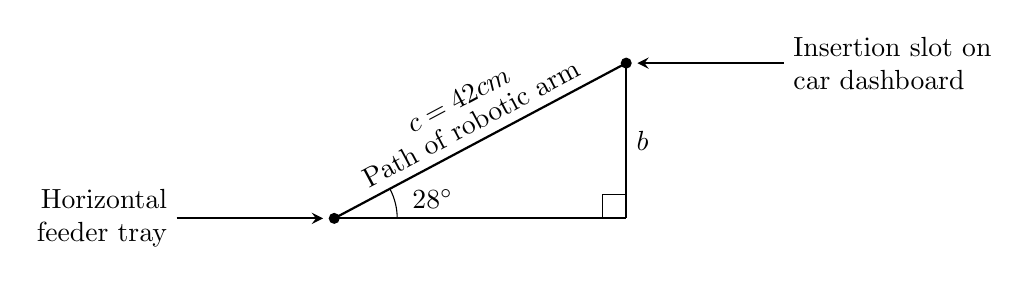
\begin{tikzpicture}
  % Define coordinates: Origin (left), Right angle (right), Top vertex
  \coordinate (A) at (0, 0);
  \coordinate (B) at ({4.2*cos(28)}, 0);
  \coordinate (C) at ({4.2*cos(28)}, {4.2*sin(28)});

  % Draw small nodes/dots at vertices A and C
  \fill (A) circle (2pt);
  \fill (C) circle (2pt);

  % Draw the triangle sides
  \draw[thick] (A) -- (B);
  \draw[thick] (B) -- (C) node[midway, right] {$b$};

  % Draw hypotenuse with both labels stacked above the line
  \draw[thick] (A) -- (C) 
    node[midway, sloped, above=10pt] {$c = 42\text{ cm}$}
    node[midway, sloped, above=0pt] {Path of robotic arm};

  % Draw the right-angle square at vertex B
  \draw (B) ++(-0.3, 0) -- ++(0, 0.3) -- ++(0.3, 0);

  % Draw the 28-degree angle arc and label at vertex A
  \draw (0.8,0) arc (0:28:0.8);
  \node at (1.25, 0.25) {$28^\circ$};

  % Corner labels placed horizontally at the exact y-coordinate of vertices
  \node (tray) at (-2.0, 0) [anchor=east, align=right] {Horizontal\\feeder tray};
  \draw[thick, ->, >=stealth, shorten >= 4pt] (tray) -- (A);

  \node (slot) at ({4.2*cos(28) + 2.0}, {4.2*sin(28)}) [anchor=west, align=left] {Insertion slot on\\car dashboard};
  \draw[thick, ->, >=stealth, shorten >= 4pt] (slot) -- (C);
\end{tikzpicture}
\end{center}

\subsection*{Trigonometric ratios in a right triangle}

Enter trigonometry!  There are three key trigonometric ratios that help us find the length of a side of a right triangle if we know the length of another side and the angles, like with Khemkhaeng's robotic arm. 

In a general right triangle, we label one angle as $\theta$ (theta, prounounced ``thay-tah'') and label the hypotenuse $c$, as usual.  Normally it doesn't matter which leg is labeled $a$ and which is $b$, but in this picture we are going to label the side opposite to (across from) $\theta$ as $b$ and the side adjacent to (next to) $\theta$ as $a$. 
\begin{center}
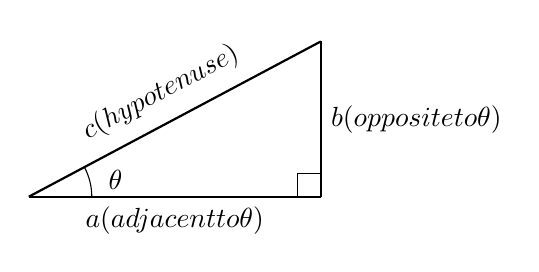
\begin{tikzpicture}
  % Define coordinates: Origin (left), Right angle (right), Top vertex
  \coordinate (A) at (0, 0);
  \coordinate (B) at ({4.2*cos(28)}, 0);
  \coordinate (C) at ({4.2*cos(28)}, {4.2*sin(28)});

  % Draw the triangle sides with descriptive labels
  \draw[thick] (A) -- (B) node[midway, below] {$a\text{ (adjacent to }\theta\text{)}$};
  \draw[thick] (B) -- (C) node[midway, right] {$b\text{ (opposite to }\theta\text{)}$};
  \draw[thick] (A) -- (C) node[midway, sloped, above=2pt] {$c\text{ (hypotenuse)}$};

  % Draw the right-angle square at vertex B
  \draw (B) ++(-0.3, 0) -- ++(0, 0.3) -- ++(0.3, 0);

  % Draw the angle arc and theta label at vertex A
  \draw (0.8,0) arc (0:28:0.8);
  \node at (1.1, 0.22) {$\theta$};
\end{tikzpicture}
\end{center}

The first trigonometric ratio is \textbf{sine}, abbreviated \textbf{sin}, is defined in a right triangle by 
$$\sin(\theta) = \frac{b}{c} = \frac{\text{opposite to } \theta}{\text{hypotenuse}}$$
The second ratio is \textbf{cosine}, abbreviated \textbf{cos}, is defined in a right triangle by 
$$\cos(\theta) = \frac{a}{c} = \frac{\text{adjacent to } \theta}{\text{hypotenuse}}$$
The third ratio is \textbf{tangent}, abbreviated \textbf{tan}, is defined in a right triangle by 
$$\tan(\theta) = \frac{b}{a} = \frac{\text{opposite to } \theta}{\text{adjacent to } \theta}$$ 

Note that $\sin(\theta)$, $\cos(\theta)$, and $\tan(\theta)$ are prounounced ``sine of theta'', ``cosine of theta'', and ``tangent of theta''. 

Whatever unit we use to measure the lengths of the sides (like cm or feet or miles) will cancel in the fractions, meaning that the sine, cosine, and tangent of an angle are just numbers without units.

A quick side note on the values of trig ratios.  First, since the legs of a right triangle are definitely shorter than the hypotenuse, each of the sine and cosine is a fraction where the top (numerator) is a smaller number than the bottom (denominator). So, the sine and cosine of any angle is always smaller than 1.  On the other hand, tangent is the ratio of the lengths of the two legs. Since either leg can be longer, the tangent can be smaller than 1 or bigger than 1, or even equal to 1 if the legs happen to be the same length.

Any scientific calculator (or other computational software) can calculate the sine, cosine, and tangent of angles.  You'll need to make sure that your calculator knows you'll be entering the angle in degrees.  (There is another way to measure angles, called radians, that is used in calculus, but we'll just use degrees in this textbook.)
For example,  check that you get $$\sin(28^\circ) = \boxed{\texttt{sin}} (28) = 0.4694715628\ldots \approx 0.4695$$

There is a mneumonic (memory tool) that people use to remember all three of these formulas
\begin{center}
    SOH-CAH-TOA
\end{center}
which is pronounced ``soh-kah-toh-uh".  Notice that S = sine, C = cosine, T = tangent, O = opposite, A = adjacent, and H = hypotenuse.  SOH-CAH-TOA doesn't really mean anything, but if you repeat it enough, you'll remember it.  

Let's use this information to answer Khemkhaeng's question. We have $$\sin(28^\circ) = \frac{b}{42}$$
If we multiply both sides of the equation by 42 we get
$$42 \times \sin(28^\circ) = \frac{b}{42}\times 42 = b$$
Rewriting the equation so that $b$ is on the left-hand side we get
$$b = 42 \sin(28^\circ) = 42 \times \boxed{\texttt{sin}} (28) = 42 \times 0.4694715628\ldots = 19.717805637\ldots \approx 19.7 \text{ cm}$$

\subsection*{Resetting the robotic arm}

Khemkhaeng needs to reconfigure the feeder layout for a new design.  The arm now needs to move 38 cm horizontally and 31 cm vertically to clear the safety sensors. At what angle (from the horizontal feeder tray) should he program the robotic arm? To begin, he draws a new picture.

\begin{center}
 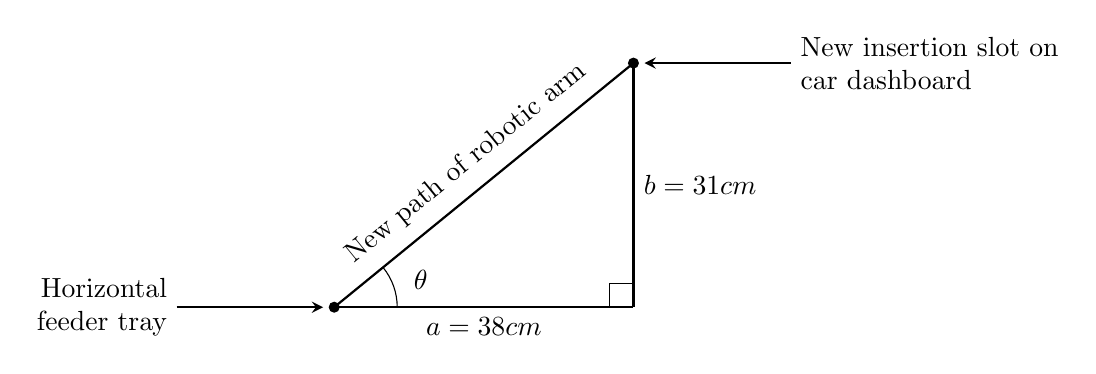
\begin{tikzpicture}
  % Coordinates scaled to match real proportions (a = 38, b = 31)
  % Angle theta = atan(31/38) ≈ 39.22 degrees
  \coordinate (A) at (0, 0);
  \coordinate (B) at (3.8, 0);
  \coordinate (C) at (3.8, 3.1);

  % Draw small nodes/dots at vertices A and C
  \fill (A) circle (2pt);
  \fill (C) circle (2pt);

  % Draw the triangle sides with updated dimensions
  \draw[thick] (A) -- (B) node[midway, below] {$a = 38\text{ cm}$};
  \draw[thick] (B) -- (C) node[midway, right] {$b = 31\text{ cm}$};

  % Draw hypotenuse labeled "Robotic arm"
  \draw[thick] (A) -- (C) 
    node[midway, sloped, above=2pt] {New path of robotic arm};

  % Draw the right-angle square at vertex B
  \draw (B) ++(-0.3, 0) -- ++(0, 0.3) -- ++(0.3, 0);

  % Draw the angle arc and theta label at vertex A
  \draw (0.8,0) arc (0:39.22:0.8);
  \node at (1.1, 0.35) {$\theta$};

  % Corner labels placed horizontally at the exact y-coordinate of vertices
  \node (tray) at (-2.0, 0) [anchor=east, align=right] {Horizontal\\feeder tray};
  \draw[thick, ->, >=stealth, shorten >= 4pt] (tray) -- (A);

  \node (slot) at ({3.8 + 2.0}, 3.1) [anchor=west, align=left] {New insertion slot on\\car dashboard};
  \draw[thick, ->, >=stealth, shorten >= 4pt] (slot) -- (C);
\end{tikzpicture}
\end{center}

Since Khemkhaeng knows the length of the side opposite to $\theta$ and the length of the side adjacent to $\theta$, he can use the tangent ratio to write an equation involving $\theta$.  He gets
$$\tan(\theta) = \frac{\text{opposite to } \theta}{\text{adjacent to } \theta} = \frac{b}{a} = \frac{31}{38} = 0.8157894737\ldots \approx 0.8158$$
How can Khemkhaeng find the angle $\theta$?

\subsection*{Inverse trigonometry in a right triangle}

Each trigonometric ratio defines a function where the independent variable is the angle (in degrees) and the dependent variable is the ratio (sine, cosine, or tangent of that angle).  Luckily, each of these functions has an \textbf{inverse} function, a way to undo it. A way to go from the ratio back to the angle.

For example, Khemkhaeng wants to undo the tangent function, so he can use the inverse tangent function. One name of this function is \textbf{arctangent}, abbreviated \textbf{arctan}.  On a calculator or computational software, the key sequence is often $\boxed{\texttt{INV}}\boxed{\texttt{tan}}$.
Since Khemkhaeng knows
$$\tan(\theta) = \frac{31}{38}$$
that means
$$\theta = \arctan\left(\frac{31}{38}\right) = \boxed{\texttt{INV}}\boxed{\texttt{tan}} ( 31 \div 38) = 39.207203505\ldots \approx 39.2^\circ$$

The other two inverse trigonometric functions are \textbf{arcsine}, abbreviated \textbf{arcsin} with key sequence $\boxed{\texttt{INV}}\boxed{\texttt{sin}}$, and \textbf{arccosine}, abbreviated \textbf{arccos} with key sequence $\boxed{\texttt{INV}}\boxed{\texttt{cos}}$. Again, you will need to make sure your calculator (or software) is working with degrees.

In precalculus and calculus textbooks, these functions often go by a strange looking names: $\arcsin(x) = \sin^{-1}(x)$, $\arccos(x) = \cos^{-1}(x)$, and $\arctan(x) = \tan^{-1}(x)$. In that context, instead of saying ``arc sine'', ``arc cosine'', and ``arc tangent'', we say ``inverse sine'', ``inverse cosine'', and ``inverse tangent''.  The superscript -1 is not a power, it is a weird but standard way to denote an inverse function.  We will stick to the arc names in this textbook.

 \input{GoDoWS}

\noindent \textbf{Do you know \ldots}

\begin{itemize}
\item How sine, cosine, and tangent are defined in a right triangle?
\item Which side is opposite to an angle and which side is adjacent to an angle in a right triangle?
\item How to evaluate sine, cosine, or tangent of an angle measured in degrees using a calculator or computational software?
\item When to use sine vs. cosine vs. tangent?
\item When to use arcsin, arccos, or arctan?
\item How to evaluate arcsin, arccos, or arctan on a calculator, making sure to be in degree?
\item How to evaluate the sine, cosine, and tangent of 30$^\circ$, 45$^\circ$, and 60$^\circ$ using special triangles?
 \input{NotSure} 
\end{itemize}

\subsection*{Exercises}

\begin{enumerate} 

\item % workbook Sine
Giraffes stretch their long necks to reach high leaves on trees.  Kirin, a giraffe at our local zoo, boasts a 6 foot long neck.  He can extend his neck at an angle of 55$^\circ$ (relative to his shoulder level) to feed on high acacia branches. If Kirin's shoulder stands 11 feet above the ground, how high a leaf can he reach?

\item % workbook Cosine and Arc cos
\begin{enumerate}
    \item A 300 foot cable is tethered from the top of a radio tower to the ground.  The cable forms a 40$^\circ$ angle with the tower. What is the height of the tower and how far away from the tower is the cable tethered to the ground?
    \item The company wants to tether another 300 foot cable to a nearby tower that is only 185 feet tall.  What angle will the cable make with the tower?
\end{enumerate}

\item %workbook  tan and arctan
Zoha wants to mount her television on the wall of her apartment. She sits down on her couch and measures two distances.  The horizontal distance from her eyes to the wall is 104" and the vertical distance from her eyes to the floor is 43".

\begin{enumerate}
    \item To prevent neck strain, Zoha wants the angle from her eyes (when she's sitting on the couch) up to the top edge of the television screen to be no more than 15$^\circ$. When she mounts the television on the wall, how many inches up the wall should the top of the screen be?
    \item Zoha's television is ``75" diagonal'', which means it is 37" tall. What is the angle from her eyes (when she's sitting on the couch) down to the bottom edge of the television screen?  
    \item To prevent neck strain, the angle you found in part (b) should also be 15$^\circ$ or less.  Is it, or should Zoha consider buying a smaller television?
\end{enumerate}

\item % workbook
In Section 7.1 we saw two special triangles that came from Tim's observations about the angles of branches of maple and linden trees in his neighborhood.  We can use those triangles to evaluate the trigonometric ratios at 30$^\circ$, 45$^\circ$, and 60$^\circ$.  Here are the two special triangles we found

\hfill
    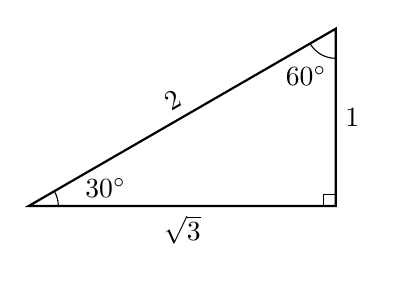
\begin{tikzpicture}[scale=.75]
    % Coordinates:
    % Side \sqrt{3} (horizontal bottom): length = 1.732 * 3 ≈ 5.196
    % Side 1 (vertical to the right): length = 3
    \coordinate (A) at (1.732*3, 0);    % Right-angle corner (bottom-right)
    \coordinate (B) at (0, 0);          % Bottom-left corner
    \coordinate (C) at (1.732*3, 3);    % Top-right corner

    % Draw Triangle
    \draw[thick] (A) -- (B) -- (C) node[midway, sloped, above] {2} -- cycle;

    % Right angle symbol (at bottom-right)
    \draw (1.732*3 - 0.2, 0) -- (1.732*3 - 0.2, 0.2) -- (1.732*3, 0.2);

    % Bottom-left 30° angle arc and label
    \draw (0.5, 0) arc (0:30:0.5);
    \node at (1.3, 0.3) {$30^\circ$};

    % Top-right 60° angle arc and label
    \draw (1.732*3, 3 - 0.5) arc (270:210:0.5);
    \node at (1.732*3 - 0.5, 2.2) {$60^\circ$};

    % Side Labels
    \node[below] at (1.732*1.5, 0) {$\sqrt{3}$};
    \node[right] at (1.732*3, 1.5) {1};
\end{tikzpicture}
\hfill
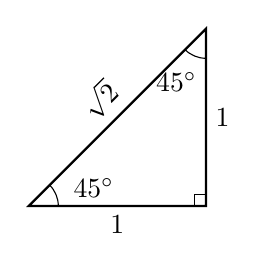
\begin{tikzpicture}[scale=.75]
    % Coordinates for 45-45-90 isosceles right triangle (legs of equal length 3)
    \coordinate (A) at (3, 0);    % Right-angle corner (bottom-right)
    \coordinate (B) at (0, 0);    % Bottom-left corner (45° angle)
    \coordinate (C) at (3, 3);    % Top-right corner (45° angle)

    % Draw Triangle with Hypotenuse Label
    \draw[thick] (A) -- (B) -- (C) node[midway, sloped, above] {$\sqrt{2}$} -- cycle;

    % Right angle symbol (at bottom-right)
    \draw (3 - 0.2, 0) -- (3 - 0.2, 0.2) -- (3, 0.2);

    % Bottom-left 45° angle arc and label
    \draw (0.5, 0) arc (0:45:0.5);
    \node at (1.1, 0.3) {$45^\circ$};

    % Top-right 45° angle arc and label
    \draw (3, 3 - 0.5) arc (270:225:0.5);
    \node at (3 - 0.5, 2.1) {$45^\circ$};

    % Side Labels
    \node[below] at (1.5, 0) {1};
    \node[right] at (3, 1.5) {1};
\end{tikzpicture}
\hfill ~
    
 \begin{enumerate}
    \item Use the first triangle to evaluate $\sin(30^\circ)$, $\cos(30^\circ)$, and $\tan(30^\circ)$.  Write your answers as exact fractions (which might involve square roots) and give decimal approximations.  Hint: The side opposite to 30$^\circ$ has length 1 while the side adjacent to 30$^\circ$ has length $\sqrt{3}$.
    \item Use the first triangle again to evaluate $\sin(60^\circ)$, $\cos(60^\circ)$, and $
    \tan(60^\circ)$.  Write your answers as exact fractions (which might involve square roots) and give decimal approximations.  Caution: The side opposite to 60$^\circ$ has length $\sqrt{3}$ while the side adjacent to 60$^\circ$ has length 1. (Lesson learned: which leg is opposite and which leg is adjacent depends on which angle we are using.)
    \item Use the second triangle to evaluate $\sin(45^\circ)$, $\cos(45^\circ)$, and $\tan(45^\circ)$.  Write your answers as exact fractions (which might involve square roots) and give decimal approximations.  Hint: the side opposite to 45$^\circ$ and the side adjacent to 45$^\circ$ each are length 1.
\end{enumerate}

\item % sine and arcsin
At a local warehouse, most of the work grabbing goods and packing them into shipping crates is done by high-speed ``pick-and-place'' robots.  Each robot works above a ramped conveyor belt that moves packages into shipping crates.  The conveyor belt has a rail that extends the robots arm horizontally to push packages up the ramp.  The standard rail goes out up to 4 feet.

\begin{enumerate}
    \item One robot is assigned a ramp that makes an angle 18$^\circ$ with the floor.  What is the height of the platform at the top of the ramp?  Assume the robot uses the full 4 foot horizontal extension from the rail.  
    \item Another robot is assigned a ramp that reaches a larger box, so the height of the platform at the top of the ramp is 30 inches.  What angle does the ramp make with the floor?  Again, assume the robot uses the full 4 foot horizontal extension from the rail.  Hint: start by converting 30 inches to decimal feet.
\end{enumerate}

\item % cosine
An airplane is getting ready to land at the airport.  Air Traffic control has authorized a descent path of 50 miles along a 3$^\circ$ glide slope, meaning the angle between the path the airplane travels and the ground is 3$^\circ$.  At what horizontal distance from the airport would the airplane begin its descent?

\item % arcsin
Rafael is a physical therapist.  His patient, a 65-year old woman, is complaining of sciatic nerve pain.
\begin{enumerate}
    \item During the intake appointment, Rafael asked his patient to lay down on the examination table and keep both her legs straight but relaxed.  Rafael lifted her right leg and stopped when the nerve pain started.  At that point, the patient's heel was 23 inches above the table.  The patient's leg is 29 inches long.  What is the hip flexion (angle) of the patient's leg relative to the table at the point where the pain starts? (By the way, this measurement is called the Straight Leg Raise (SLR) test.)
    \item After 6 weeks of physical therapy, Rafael repeated the assessment.  The goal is to be able to get his patient's leg to to 70$^\circ$ hip flexion (angle) without pain.  How high off the table would Rafael need to lift his patient's heel without pain to to reach this goal?
\end{enumerate}

\item % tangent
An oceanographic survey ship uses sonar (sound) to map a deep-sea trench. The sonar beam is aimed at an underwater ridge at an angle of $35^\circ$ measured from the vertical line dropping directly down from the ship. The ridge is located at a horizontal distance of 840 meters from the ship.
\begin{enumerate}
    \item What is the depth of the ocean floor at the ridge?
    \item If another trench section is known to be \text{1,500} meters deep, at what angle from the vertical should the team direct their sonar beam to hit a feature 900 meters horizontally away?
\end{enumerate}

\end{enumerate}

\bigskip

\noindent \textbf{When you're done \ldots}

\begin{itemize}
\item Don't forget to check your answers with those in the back of the textbook. 
\item Not sure if your answers are close enough? Compare with a classmate or ask the instructor.  
\item Getting the wrong answers or stuck on a problem?  Re-read the section and try the problem again.   If you're still stuck, work with a classmate or go to your instructor's office hours.
\item It's normal to find some parts of some problems difficult, but if all the problems are giving you grief, be sure to talk with your instructor or advisor about it.  They might be able to suggest strategies or support services that can help you succeed.
\item Make a list of key ideas or processes to remember from the section.  The ``Do you know?'' questions can be a good starting point.
\end{itemize}



